\begin{comment}
\section{Comparison of basic and ensemble approaches}
\label{sec:transfer-comparison}

The different approaches were compared using cross-validation Average Precision (AP) to assess whether ensemble methods improve upon the basic classifiers. Model selection also considers the requirements of the real-world application, where interpretability and practical usefulness are important alongside predictive performance.

Transfer learning was considered but not included in the final model comparison. No suitable publicly available models or datasets from comparable universities were found. We also explored splitting the dataset by academic programme, pretraining on the other programmes and fine-tuning on the largest
one, but this gave no clear gain over training from scratch. These groups come from the same institution and share all features, so they are not sufficiently distinct domains. We therefore focused on conventional supervised
learning and ensemble methods.

\begin{figure}[H]
    \centering
    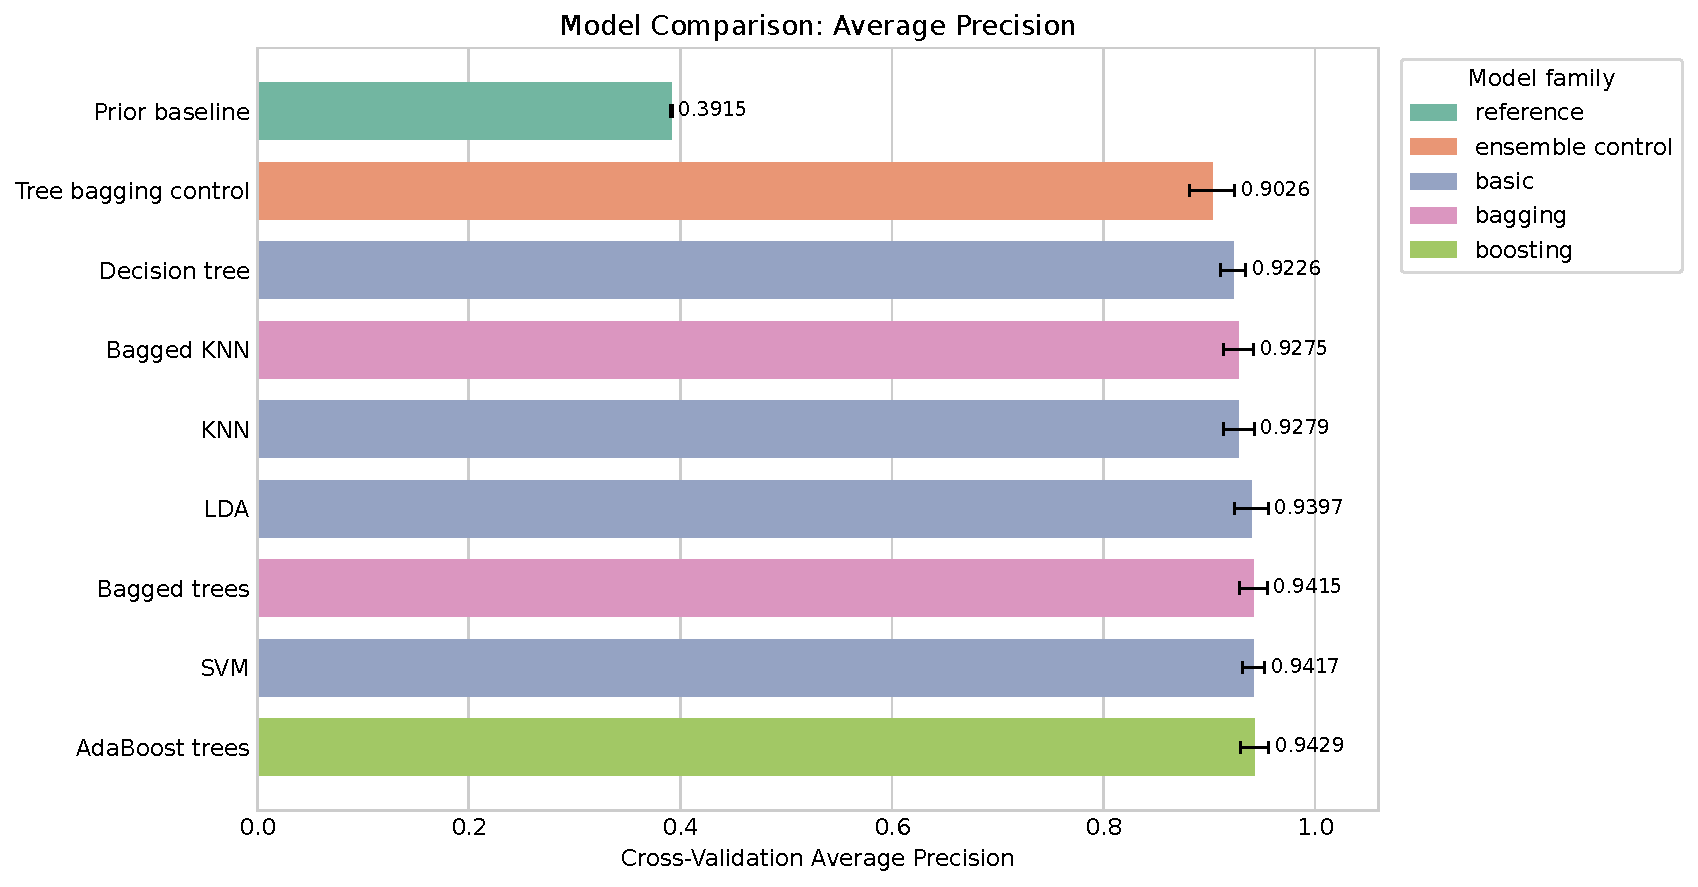
\includegraphics[width=0.9\textwidth]{Images/08_model_comparison_AP.pdf}
    \caption{Comparison of basic classifiers, ensemble methods and the single decision tree control using cross-validation average precision. Error bars indicate one standard deviation across folds.}
    \label{fig:model-comparison-ap}
\end{figure}

\subsection{Performance comparison}

Figure~\ref{fig:model-comparison-ap} shows that AdaBoost achieved the highest AP of 0.9429, closely followed by SVM (0.9417), bagged decision trees (0.9415) and LDA (0.9397).

Both boosting and bagging improved decision tree performance. AdaBoost increased AP from 0.9226 to 0.9429, while bagging increased it to 0.9415 compared to the single decision tree
control. This suggests that combining multiple trees can improve predictive performance compared to an individual
tree.

In contrast, bagging KNN provided no improvement, with AP decreasing slightly from 0.9279 to 0.9275. This indicates
that the benefits of ensemble methods depend on the underlying classifier.

Although AdaBoost achieved the highest score, its advantage over LDA was only 0.0031. Given the intended use of supporting academic advisors, this marginal improvement may not justify the additional model complexity. LDA offers a simpler alternative, with coefficients that can be examined to understand how features contribute to predictions.



\end{comment}
% ----------------------------------------------------




\section{Comparison of basic and ensemble approaches}
\label{sec:transfer-comparison}

The basic, ensemble and LDA workflows were compared on the same five stratified
group folds. Mean validation average precision (AP) selects settings within
each model family. For the final recommendation, we also consider performance
within the 20\% advisor contact budget and how readily the model can be explained.

Transfer learning is outside our chosen problem scope. We develop one ranking
model for the pooled student population, with labelled training data available
for that population. Adapting a model to a new institution or a programme with
little labelled data would address an additional question. We therefore focus
on conventional supervised learning and ensemble methods.

\subsection{LDA classifier}
\label{sec:lda-classifier}

Here LDA directly classifies \texttt{Dropout} versus \texttt{Graduate}, unlike
the LDA projection followed by
logistic regression in Section~\ref{sec:feature-selection}.
Eight configurations combine retained predictors with or without 11 engineered
features and four covariance options: no shrinkage with the \texttt{svd} solver,
or automatic, 0.1 or 0.5 shrinkage with \texttt{lsqr}. Shrinkage stabilizes the
covariance estimate for correlated predictors~\cite{sklearn_lda}.
Encoding, scaling and constant-feature removal are fitted within each training
fold. Mean AP across the same five stratified group folds selects engineered
features, \texttt{lsqr} and automatic shrinkage. The model fitted on all 2,904
development students has 114 preprocessed inputs, 114 coefficients and one
intercept. Its F2-selected alert cutoff is described in
Section~\ref{sec:final-evaluation}.

\subsection{Performance comparison}

\begin{figure}[H]
    \centering
    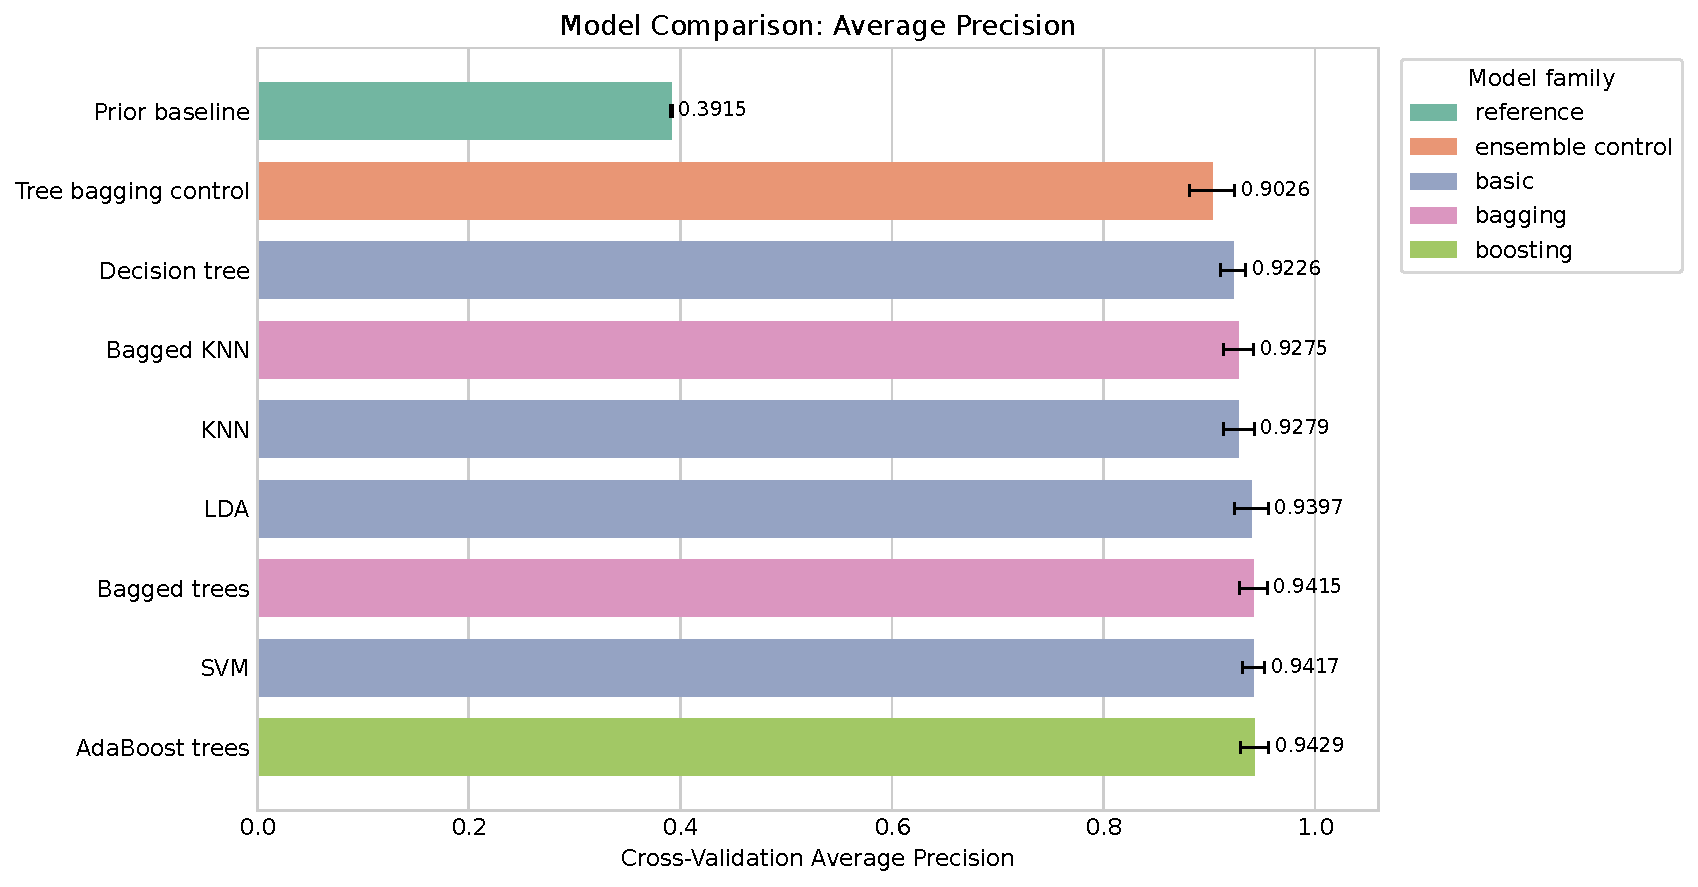
\includegraphics[width=\linewidth]{Images/08_model_comparison_AP.pdf}
    \caption[Validation AP across model families]{Mean AP across the same five
    development folds. Error bars show one standard deviation across folds,
    not confidence intervals. These are validation results used for tuning.}
    \label{fig:model-comparison-ap}
\end{figure}

AdaBoost achieved the highest mean validation AP, 0.9429, followed by SVM
(0.9417), bagged trees (0.9415) and LDA (0.9397)
(Figure~\ref{fig:model-comparison-ap}). AdaBoost improved on the tuned basic
tree's AP of 0.9226, while tree bagging improved on its matched single-tree
control's 0.9026. Bagged KNN did not improve on basic KNN, with AP changing
from 0.9279 to 0.9275. Averaging can stabilize individual trees, while KNN
already averages neighbours and need not benefit from further averaging.
Different feature sets and tuning budgets mean these are workflow comparisons.
At the 20\% contact budget, LDA and AdaBoost each found 580 recorded dropouts
among 581 selected development students using pooled out-of-fold predictions.
They reached the same number of cases, although their contact lists differed.

For advisor prioritisation, we prefer LDA because its linear score makes
feature contributions easier to inspect than AdaBoost's 80-tree ensemble.
We accept the small loss in validation AP in exchange for this explainability
when the contact yield is the same. This establishes the model preference
from development results. Section~\ref{sec:final-evaluation} evaluates test
performance and compares complexity, computation time and advisor workload.
